\PassOptionsToPackage{subsection=false}{beamerouterthememiniframes}
% the above removes the subsection bar

\documentclass[11pt]{beamer}
\usetheme{Amsterdam}
\setbeamercolor{subsection in head/foot}{fg=White}
%\usetheme{CEA}

\usepackage{lmodern}
\usepackage{multirow}

\usepackage[T1]{fontenc}

\usepackage[utf8]{inputenc}

\usepackage{graphicx} 

%\usepackage{hyperref}

\usepackage{tikz}
\usetikzlibrary{positioning,patterns,matrix,calc,arrows,shapes,fit,decorations.pathmorphing}


\usepackage{amsmath}
\usepackage{amsfonts}
\usepackage{amssymb}
\usepackage{color}
\newtheorem{thm}{Theorem}
\newtheorem{cor}{Corollary}

\usepackage{algorithm}
\usepackage{algpseudocode}

\usepackage{xspace}
\usepackage{hyperref}

\newcommand{\msl}{\{\hspace*{-0.1cm}|}
\newcommand{\msr}{|\hspace*{-0.1cm}\}}

\definecolor{olivegreen}{RGB}{85, 107, 47}
\definecolor{purple}{RGB}{128, 0, 128}
\definecolor{darkviolet}{RGB}{148, 0, 211}
\newcommand{\mg}[1]{{\color{magenta} #1}}
\newcommand{\cyan}[1]{{\color{cyan} #1}}
\newcommand{\olive}[1]{{\color{darkviolet} #1}}
\newcommand{\red}[1]{{\color{red} #1}}


\renewcommand{\algorithmiccomment}[1]{\hfill\  #1}
\renewcommand{\algorithmicrequire}{\textbf{Input:}}
\renewcommand{\algorithmicensure}{\textbf{Output:}}



\title{Enhancing public key infrastructure with blockchain}

%\institute{institute/whatever}

\date{}

%pages enumeration
\setbeamertemplate{footline}[text line]{%
  \parbox{\linewidth}{\vspace*{-8pt}
  REDOCS 2018 \hfill\insertframenumber / \inserttotalframenumber}}
\setbeamertemplate{navigation symbols}{}


%\addtobeamertemplate{frametitle}{\vskip-1.5ex}{}



\AtBeginSection[]
{
  \begin{frame}<beamer>
    \tableofcontents[currentsection]
  \end{frame}
}

\beamertemplatenavigationsymbolsempty
\begin{document}
%\beamertemplatenavigationsymbolsempty

\author{%
\begin{tabular}{rl}
Fabien Charmet & T\'{e}l\'{e}com SudParis, Institut Mines-T\'{e}l\'{e}com,\\
& CNRS Samovar UMR 5157\\
Maxime Montoya & Univ. Grenoble Alpes, CEA, LETI, DACLE\\
Mathieu Valois & Normandie Univ, UNICAEN, ENSICAEN,\\
& CNRS, GREYC\\
Wojciech Wide\l{} & Univ Rennes, INSA Rennes, CNRS, IRISA\\
\end{tabular}
%\vspace{2mm}
\center
26 October 2018}


%\maketitle

\begin{frame}

\titlepage

\vspace{-19mm}
\begin{center}
\begin{tabular}{l @{\hspace{35mm}} r}

\includegraphics[scale=0.14]{redocs_logo2}
&

\includegraphics[scale=0.14]{idnomicLogo} 
\end{tabular} 
\end{center}
\end{frame}


\begin{frame}
context here:
what is it that we are trying to achieve/what IDNOMIC wants + threat model description
\end{frame}


\begin{frame}
titles:

Blockchain-based enhancements of public key infrastructure

Enhancing public key infrastructure with blockchain

Improving PKI with blockchain

Towards a decentralized identity management solution based on blockchain

or something else
\end{frame}


\begin{frame}{Outline}
\tableofcontents
\end{frame}


\section[PKI and blockchains]{Background on public key infrastructure (PKI) and blockchains}


\begin{frame}{Public-key encryption}
\begin{center}
\begin{tikzpicture}
[node distance=2cm and 0.5cm]
% 'd' for dummies
% upper level: r  sk  d pk d5
% lower level: d2 d3 ct d4 pt s

% lower
\node[label=above:{Recipient}](r) {{\LARGE \faUser}};

\node[right = of r.east] (d3) {decrypt};

\node[right = of d3.east, label=below:{ciphertext}] (ct) {{\Huge \faFileText}};

\node[right = of ct.east] (d4) {encrypt};

\node[right = of d4.east, label=below:{plaintext}] (pt) {{\Huge \faFileTextO}};

\node[right = of pt.east, label=above:{Sender}](s) {{\LARGE \faUser}};

% upper

\node[above = of d3.north, label=above: {secret key}] (sk) {{\Huge \red{\faKey}}};

\node[above = of d4.north, label=above: {public key}] (pk) {{\Huge \olive{\faKey}}};


%\node[](r) {Recipient:};
%
%\node[right = of r.east, label=above: {secret key}] (sk) {{\Huge \red{\faKey}}};
%
%\node[right = of sk.east] (d) {};
%
%\node[right = of d.east, label=above: {public key}] (pk) {{\Huge \olive{\faKey}}};
%
%\node[right = of pk.east] (d5) {};

%horizontal upper
%\draw[->] (r) to (sk);

%vertical
\draw[->] (pk) to (d4);
\draw[->] (sk) to (d3);
%\draw[->] (d2) to (r);

%horizontal lower
\draw[-] (s) to (pt);
\draw[-] (pt) to (d4);
\draw[->] (d4) to (ct);
\draw[-] (ct) to (d3);
\draw[->] (d3) to (r);

\end{tikzpicture}
\end{center}

%{\large test test}
%
%{\LARGE test test}
%
%{\LARGE \faKey}
\end{frame}

\begin{frame}{Public key infrastructure}

\begin{itemize}
\item \mg{Public key infrastructure (PKI)}: a set of roles, policies, and procedures needed to
%create, manage, distribute, use, store, and revoke
%digital certificates and manage public-key encryption.
ensure
secure distribution of public keys
\item Based on digital certificates
\end{itemize}


%'digital certificate = signature
%binding an entity to some public key'

%\vspace{2mm}
%
%PKI involves
%\begin{itemize}
%\item public key cryptography,
%\item digital certificates,
%\item digital identity management.
%\end{itemize}

\end{frame}


\begin{frame}{Digital certificate}
%based on https://tex.stackexchange.com/a/8935
\begin{center}
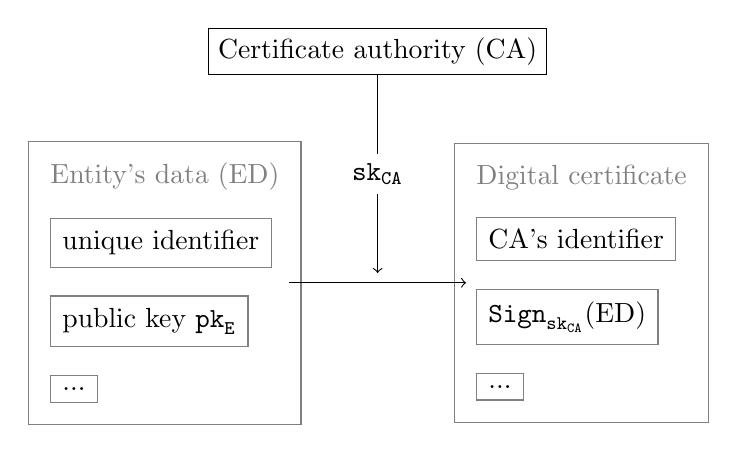
\begin{tikzpicture}[mymatrix/.style={matrix of nodes, nodes=typetag, row sep=1em},
  mycontainer/.style={draw=gray, inner sep=1ex},
  typetag/.style={draw=gray, inner sep=1ex, anchor=west},
  title/.style={draw=none, color=gray, inner sep=0pt}
  ]
  \matrix[mymatrix] (user) {
    |[title]|Entity's data (ED)\\
    unique identifier\\
    public key $\mathtt{pk}_{\mathtt{E}}$ \\
    ... \\
  };
  
  \node[right=of user.east] (fake) {};
  
  \node[above = of fake] (fakeN) {$\mathtt{sk}_{\mathtt{CA}}$};
  
  \node[draw,rectangle,
fill=white, above = of fakeN](ca) {Certificate authority (CA)};
  
    \matrix[mymatrix, right=of fake.east, matrix anchor=west] (cert) {
    |[title]|Digital certificate\\
    CA's identifier\\
    $\mathtt{Sign}_{\mathtt{sk}_{\mathtt{CA}}}($ED$)$\\
    ...\\
  };
  
  \node[mycontainer, fit=(user)] {};
  \node[mycontainer, fit=(cert)] {};
  \draw [->] (user) to (cert);
  \draw [-] (ca) to (fakeN);
  \draw [->] (fakeN) to (fake);
  
\end{tikzpicture}
\end{center}
\pause
\begin{center}
CA certifies: $\mathtt{pk}_{\mathtt{E}}$
is indeed the public key of the entity
\end{center}
\end{frame}


%\begin{frame}{Public key infrastructure}
%\begin{figure}[t]
%\begin{tikzpicture}
%\node[draw,rectangle,
%inner xsep=1cm,inner ysep=1cm,
%label=below:{entity's data},
%fill=white](user) at (-30,0){};
%
%\node[] (fake) at (-28,0){};
%
%\node[draw,rectangle,
%fill=white](ca) at (-28,2){Certificate authority (CA)};
%
%\node[draw,rectangle,
%inner xsep=1cm,inner ysep=1cm,
%label=below:{digital certificate},
%fill=yellow](cert) at (-26,0){};
%
%\node[draw,rectangle,
%inner xsep=1cm,inner ysep=1cm,
%fill=green](repo) at (-22,0){};
%
%
%\draw [->] (user) to (cert);
%\draw [->] (cert) to (repo);
%\draw [->] (ca) to (fake);
%\end{tikzpicture}
%\end{figure}
%
%a figure to be placed here, based on IDNOMIC's page 6
%\end{frame}


\begin{frame}{Public key infrastructure}

chain of trust, revocation of certificates

\end{frame}

\begin{frame}{Blockchain definition}

\begin{itemize}
\item \mg{Blockchain}: a public, transparent,
append-only ledger
%\pause
\item Created by members of a peer-to-peer
network
\item Immutable and unforgeable records (\mg{blocks})
%Records \mg{blocks} stored in the ledger are immutable
%and unforgeable
\item FunFactHere?
\end{itemize}

\end{frame}



\begin{frame}{Blockchain structure}

\begin{itemize}
\item \mg{Transaction}: atomic event
allowed by the blockchain protocol (`Alice sends Bob $0.1$ BTC')
\item Transactions are \mg{validated} and \mg{broadcast}
throughout the network.
\item Validated transactions
stored in \mg{blocks}
\item Blocks linked together,
forming a \mg{chain}
\item The choice of the next blocks to be
added to the chain is a result of a \mg{consensus
process}
\end{itemize}

\end{frame}

\begin{frame}{Blockchain structure}

\begin{center}
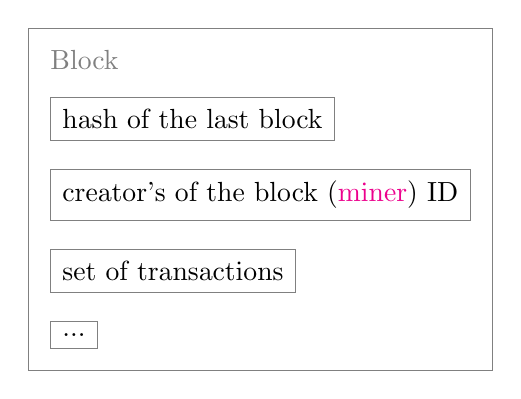
\begin{tikzpicture}[mymatrix/.style={matrix of nodes, nodes=typetag, row sep=1em},
  mycontainer/.style={draw=gray, inner sep=1ex},
  typetag/.style={draw=gray, inner sep=1ex, anchor=west},
  title/.style={draw=none, color=gray, inner sep=0pt}
  ]
  \matrix[mymatrix] (block) {
    |[title]|Block\\
    hash of the last block\\
    creator's of the block (\mg{miner}) ID\\
    set of transactions\\
    ...\\
  };
  
  
  \node[mycontainer, fit=(block)] {};
  
\end{tikzpicture}
\end{center}

\end{frame}


\begin{frame}{Blockchain structure}

\begin{center}
\begin{tikzpicture}

  \node[draw,rectangle,
fill=white, label=below:{Genesis block}](gb) {Block 0};

  \node[draw,rectangle,
fill=white, right = of gb](b1) {Block 1};

  \node[right = of block.east, label=below:{...}] (dots) {};
  
    \node[draw,rectangle,
fill=white, right = of dots](bl) {Block $n$};

  \node[right = of bl.east] (dummy) {};
  
%  \node[above = of dummy.north] (dummy2) {};
%  
%  \node[below = of dummy.north] (dummy3) {};
  
%   \node[draw,rectangle,
%fill=white, right = of dummy2](nb1) {Block?};
%
%   \node[draw,rectangle,
%fill=white, right = of dummy3](nb2) {Block???};

   \node[draw,rectangle,
fill=white, right = of bl.north east](nb1) {Block?};

   \node[draw,rectangle,
fill=white, right = of bl.south east](nb2) {Block???};
  
  
  \draw [->] (gb) to (b1);
  \draw [->] (b1) to (dots);
  \draw [->] (dots) to (bl);
  \draw [->] (bl) to (nb1);
  \draw [->] (bl) to (nb2);
  
\end{tikzpicture}
\end{center}

ugly, to be modified

\end{frame}

\section[Blockchains for PKI]{How blockchains could enhancing PKI}

\begin{frame}{Blockchain and Man-in-the-middle attacks}
	\begin{alertblock}{Attacks}
		\begin{itemize}
			\item Hack of genuine certification authorities
			\item CA producing certificates for domains they don't own (Iran with Google)
		\end{itemize}
	\end{alertblock}

	\begin{exampleblock}{Blockchain}
		\begin{itemize}
			\item \mg{transparency} and \mg{traceability}
			\item Secure distributed log that cannot be altered
			\item The whole chain of trust is stored
		\end{itemize}
	\end{exampleblock}
\end{frame}

\begin{frame}{Blockchain and Certificate Revocation Lists}
	\begin{alertblock}{Current issues}
		\begin{itemize}
%			\item Updated periodically but not instantly
			\item Separated process to check CRLs for end users: adds delays, and is not performed at all by some web browsers
		\end{itemize}
	\end{alertblock}

	\begin{exampleblock}{Blockchain solution}
%		\mg{Faster} and \mg{more secure} verification of revocations
		\begin{itemize}
%			\item CRLs are updated instantaneously
			\item All CRLs stored at the same place
			\item CRLs checked together with certificates in one single query
		\end{itemize}
	\end{exampleblock}
\end{frame}

\begin{frame}{Examples of applications of blockchains to PKIs}

	\begin{exampleblock}{Trusted domain names}
		\begin{itemize}
			\item Privacy and confidentiality issue: are visited websites what they pretend to be ?
			\item Millions of certificates, with variable lifetime
		\end{itemize}
	\end{exampleblock}
	
	\begin{alertblock}{Trusted connected cars}
		\begin{itemize}
			\item Safety issue: connected or even autonomous cars might need to check that the surrounding cars are legitimate
			\item Thousands of certificates, with a one-week lifetime
		\end{itemize}
	\end{alertblock}

%\emph{In both cases, all certificates and CRLs would be stocked together in a blockchain.}

\end{frame}

\section[Storing certificates on a ledger]{Storing certificates and
certificate revocation lists on a blockchain ledger}

\begin{frame}
task: enhance PKI by storing certificates
and CRL
in a blokchain ledger

recall the assumptions/threat model
\end{frame}

\subsection[subsec1]{Possible approaches}

\begin{frame}
possible solutions:

- ethereum's smart contracts

- bitcoin's op\_return

- multichain
\end{frame}

\subsection[subsec2]{Our solution}

\begin{frame}
frame
\end{frame}

\section[Demonstration]{Demo}

\begin{frame}
	\frametitle{Demo}
	\begin{center}
		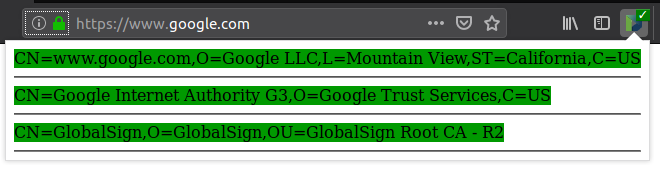
\includegraphics[scale=0.4]{figs/green_certs.png}
		
\includegraphics{figs/green_tick.png}
	\end{center}
\end{frame}

\begin{frame}
	\frametitle{Demo}
	\begin{center}
		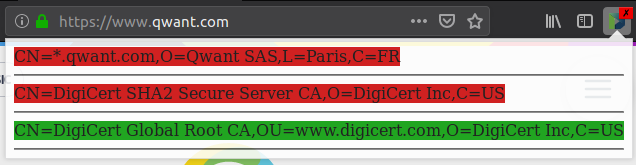
\includegraphics[scale=0.4]{figs/red_certs.png}
		
\includegraphics{figs/red_mark.png}
	\end{center}
\end{frame}


\end{document}